% Die Vorlage fuer Abschlussarbeiten benutzt die hervorragende
% Klasse ``hepthesis'' von Andy Buckley
% zusammengestellt von : Felix Richter, 02.03.2010

%\documentclass[12pt,twoside,bind,ams,a4paper,hyper]{hepthesis}
\documentclass[12pt,twoside,bind,ams,a4paper]{hepthesis}

% Unicode(UTF-8)-Kodierung anschalten. Damit koennen dann alle
% deutschen Umlaute und fremdsprachlichen Zeichen direkt verwendet werden (z.B. - statt \"A)
% es muss allerdings ein unicode-faehiger Editor benutzt werden (unter Linux alle, unter Windows ???).
\usepackage[utf8]{inputenc}
\usepackage[T1]{fontenc}
% fuer eine Arbeit in deutscher Sprache sinnvoll:
\usepackage[ngerman, english]{babel}
% Schriftarten: Variante 1
\usepackage{lmodern,hfoldsty,charter}
% Schriftarten: Variante 2
%\usepackage{charter}
% Paket fuer mathematische Symbole
\usepackage{amssymb}

% Paket fuer Literaturverzeichnis nach DIN
\usepackage{natbib}
% Literaturzitate in eckige Klammern setzen
\setcitestyle{square}

% Paket zum Einbinden von ein- oder mehrseitigen PDFs
\usepackage{pdfpages}

\usepackage{url}

% Paket zur typographisch richtigen Angabe von Groessen mit SI-Masseinheiten
\usepackage[squaren]{SIunits}

% Paket fuer Bra-/Ket-Vektor-Schreibweise, mit automatischer Groessenanpassung
\usepackage{braket}

% New packages
\usepackage{multirow}

% Neue Kommandos
\newcommand{\dps}[1]{\displaystyle{#1}}
\newcommand{\eq}[1]{({\ref{#1}})}
\newcommand{\fig}[1]{Fig.~{\ref{#1}}}
\newcommand{\tab}[1]{Tab.~{\ref{#1}}}
\def\dd{\text{d}}
\newcommand{\mean}[1]{\left\langle #1 \right\rangle}
\newcommand{\partder}[2]{\dfrac{\partial {#1}}{\partial {#2}}}
\newcommand{\frstder}[1]{\dfrac{\partial}{\partial {#1}}}
\newcommand{\comma}{\; , \quad}
\newcommand{\point}{\quad .}

\title{Suspended Sediment Transport near Sloping Topography}
\author{Kirstin Schulz}

% Die folgenden Zeilen aktivieren, wenn ein PDF mit anklickbarem Inhaltsverzeichnis
% sowie anklickbaren Verweisen auf Gleichungen und Literaturhinweise erzeugt werden soll.
% Die folgenden Zeilen auskommentieren, wenn ein PDF zum reinen Ausdruck erzeugt werden soll.
% Zusaetzlich muss oben im documentclass-Befehl, die Option ``hyper'' herausgenommen  
% bzw. hinzugefuegt werden.
%\hypersetup{
% pdfauthor = {\theauthor},
% pdftitle = {\thetitle},
% pdfsubject = {Master's thesis, University of Rostock, Germany, 2010},
% bookmarksopen=true
%}


% Zeilenanstaende -- eins der folgenden auswaehlen. 1 1/2 ist Voreinstellung, sollte 
% beibehalten werden.

%\setmainmatterspacing{single}
%\setmainmatterspacing{onehalf}
%\setmainmatterspacing{double}

\begin{document}

\begin{frontmatter}
% ``klassisches'', vollstaendig in Latex gesetztes Titelblatt
% Klassische Titelseite

\thispagestyle{empty}
\begin{center}
\vspace*{-2cm}
\includegraphics[width=0.75\textwidth]{unilogo-siegel-farbe}\\
\vspace*{3cm}
    {\titlefont \huge \onehalfspacing
	\thetitle 
    \par}%
   \vfill
%  \vskip 6em
    {\normalfont\normalcolor\bfseries
	\large
	Dissertation \\
	\large
%	im Studiengang Physik\\
	zur\\
	Erlangung des akademischen Grades\\
	doctor rerum naturalium (Dr. rer. nat.)\\ 
	der Mathematisch-Naturwissenschaftlichen Fakultät\\
	der Universität Rostock
    \par}%
\end{center}\par
%\vfill
\vspace*{2.5cm}
\noindent\begin{minipage}[b]{\textwidth}
{\bf
  \noindent vorgelegt von\\
  Kirstin Schulz, geb.~am 10.~Januar 1988 in 
Clausthal-Zellerfeld\\

%%% Nur für Pflichexemplare

%  \begin{tabbing}
%  Betreuer und 1.~Pr\"ufer :  \= PD Dr. Lars Umlauf, Leibniz Institut für 
%Ostseeforschung\\
% 2.~Pr\"ufer: \> ???, Universität Rostock \\
%  \end{tabbing}

  \noindent Rostock, den  1.~April 2010
  }
\end{minipage}




% Alternative: Titelblatt im Uni-Corporate-Design aus Word/OpenOffice-Vorlage erstellen,
% als PDF abspeichern/exportieren und hier mit pdfpages einbinden.
% \includepdf[pages={1}]{titelseite-cd.pdf}


\begin{abstract}[Abstract]
\thispagestyle{plain}
Sediment transport is governed by the complex interplay of many different 
processes. Near sloping topography, sediment transport can be triggered by 
asymmetries in the density stratification during an oscillatory current going 
up and down the slope. This process was investigated in detail by means of an 
idealized numerical model. It was found that the process depends on the 
strength of the vertical stratification and the slope angle, and residual 
sediment transport is directed upslope for most of the parameter constellations. 
A more profound numerical model was used to successfully reproduce observations 
of this process from the East China Sea, and to investigate the effect of Earth 
rotation. Another data set was analyzed to investigate the transport of sediment 
across the rim of a deep basin in the Baltic Sea. It was found that parts of 
the sediment transported there are dispersed across the bottom slope into 
shallower areas.
\end{abstract}


\begin{abstract}[Zusammenfassung]
\thispagestyle{plain}
\sloppy
Der Transport von Sedimenten wird von dem komplexen Zusammenspiel vieler 
verschiedener Prozesse bestimmt. Nahe eines geneigten Meeresbodens können 
Asymmetrien in der vertikalen Dichteschichtung während der Phasen einer 
oszillierenden Strömung quer zum Hang einen residuellen Sedimenttransport 
verursachen. Dieser Prozess wurde mit der Hilfe eines idealisierten numerischen 
Modells detailliert untersucht. Es hat sich gezeigt, dass die Stärke der 
vertikalen Dichteschichtung und der Winkel des Hanges eien großen Einfluss auf 
diesen Prozess haben, der residuelle Sedimenttransport aber für den Großteil 
der Parameterkombinationen hangaufwärts gerichtet ist. Das Model wurde 
erweitert, um erfolgreich Beobachtungen dieses Prozesses aus dem 
Ostchinesischen Meer zu reproduzieren und um den Einfluss der Erdrotation zu 
untersuchen. Ein weiteres Datenset wurde analysiert um den Sedimenttransport 
am Hang eines tiefen Beckens in der Ostsee zu untersuchen. Es wurde 
herausgefunden, das Sediment, welches einmal in das Becken hinein transportiert 
wurde, auch wieder in Richtung flacherer Gebiete verteilt werden kann.
\fussy
\end{abstract}
%\cleardoublepage%

\newpage
\thispagestyle{plain}
\begin{center}
 \textbf{Acknowledgements}
\end{center}

I like to express my deep gratitude to the people who surrounded and supported 
me during my PhD time. In the last three years I did not only get to know a 
totally new field of scientific work, but I met unbelievably wonderful 
people that made my time in Rostock to be a great experience. 

In first place, I thank my supervisor Lars Umlauf, who invested so much time 
and energy to make a physicist out of me. Thank you for encouraging me all the 
time and thank you for all your advice, and for helping me through the hard 
times when nothing went right.

I also thank the other three members of my thesis committee: Hans Burchard, 
thank you for introducing me to all the people on the conferences and for 
always offering your help. You were like a second supervisor for me. Henk 
Schuttelaars, thank you for all the wonderful conversations, in Havard as well 
as on the Christmas Market, and your advice on my work and my future. And 
finally Gregor Rehder, who was the most sympathetic chief scientist I ever went 
on a cruise with. 

I greatly thank my working group and the colleagues from the project. Thanks 
to all the people that shared some time in room 214 with me: Mahdi 
Mohammadi-Aragh, who helped me so much during my first time and provided me with 
the most important schedule ever, Kaveh Purkiani and Johannes Becherer, Merten 
Siegfried, Selina Müller and Madline Kniebusch, who all contributed to the 
familiar and relaxed atmosphere in our office. Special thanks goes to Chris 
Lappe, who untiringly answered all my questions about oceanography and who tried 
to explain internal waves to me at least a hundred times. Thanks to GETMan Knut 
Klingbeil, for permanent support with everything related to computers, and for 
your ability to encourage me. Thanks to Elisabeth Schulz, who I always looked up 
to. Thanks to Peter Holtermann for showing me Galvano, to Ulf Gräwe, 
Xaver Lange and Berkay Basdurak for providing support and a wonderful and 
relaxed working atmosphere. Thanks to Berit Recklebe for being the shield to 
protect me from administration and for being a friend from my first working day 
on. I also want to thank Toralf Heene and Sebastian Beier for the technical 
support and their patience with me, and of course the crew members of the 
research vessels Alkor, Elisabeth Mann Borgese and Maria S. Merian. Thanks to 
Claudia Morys, Dennis Bunke, Jana Wölfel, Mayya Gogina, Florian Cordes and Julia 
Regnery, who made the ships cruises an unforgettable experience and became my 
closest friends during my time in Rostock.\newpage
\thispagestyle{plain} I am so grateful that I had the opportunity to meet all of 
you and I hope we will stay in touch.

I also want to express my gratitude to Prof. Dr. Margit Rösler, who was my 
mentor during my years at the Technical University of Clausthal-Zellerfeld, and 
who taught me to never surrender to a problem. I would also like to thank 
Wiebke Klünder and Markus Schreiber for always being there for me, during study 
times and beyond.

In the end, I want to thank my perfect flatmate Josephina Seltenheim, for 
providing me shelter when I came to Rostock and for being such a wonderful 
person, and all my other friends in Berlin. I always loved to have you around. 
I want to thank my best friend Jennifer Smoch for your endless support with 
anything and the wonderful times we have together and my partner Christian 
Meier for his patience and for moving to the Netherlands with me. I thank my 
family, my grandmother Eva Eggeling and especially my mother and friend Maike, 
for creating a wonderful childhood for me and for supporting me in every 
possible way. Everything I have achieved so far I owe to you. I thank my amazing 
brother Paul for all the years we have been together and my father Uwe for 
everything he did for me. Finally, I particularly want to thank Marko 
Lipka, who shared his apartment, Socke the dog and his small family with me for 
the last two years. You and Klara were such a huge and wonderful part of my 
life here and I will miss you so much. Goodbye und Guten Flug. 

\textbf{Regarding the publication in chapter 2:} This study was carried out in 
the context of the
interdisciplinary project SECOS, funded by the German Federal Ministry
of Education and Research under grant 03F0666A, WP 2.1 (PI: Lars
Umlauf). We are grateful to Henk Schuttelaars (TU Delft), Hans
Burchard, Ulf Gr{\"a}we, and Knut Klingbeil (all IOW) for modeling
support and helpful comments on the manuscript. Computations were
carried out with a modified version of General Ocean Turbulence Model
(GOTM, www.gotm.net) with the SPM component implemented using the
Framework for Aquatic Biogeochemical Models (FABM,
www.sf.net/projects/fabm).
\newpage

\tableofcontents

\end{frontmatter}

\begin{mainmatter}
\chapter{Introduction}
\label{kap-intro}

% Seitennummerierung auf arabische Zahlen umstellen, neu beginnend im Kapitel 1
\pagenumbering{arabic}

%\chapterquote{Dämliches Zitat}{Zitierter Mensch}

Motivation

Outline Diss.
\chapter{Sediment transport over sloping topography}
\label{kap-slope}

\section{Motivation}

To investigate basin scale sediment transport pathways, a distinct knowledge about the underlying, small scale processes is crucial. Motivated by the outcomes of studies on estuarine dynamics, which trigger sediment transport processes, a basic process study was carried out. The impact of an oscillatory current moving over sloping topography with overlying stratified water body on suspended matter transport was examined. 

The basin structure and the permanent salinity stratification provide the requirements for the above process in large areas of the Baltic Sea. Although tides do not play a significant role, other oscillatory currents are found in the Baltic: near-inertial waves, internal seiching motions in the basins, topographic \citep[][]{holtermann2012} or coastal-trapped waves \citep[][]{pizarro1998}.

In the absence of tides and due to the permanent deep-water stratification, inertial oscillations and low-mode near-inertial wave motions have been found to dominate the energetics on the basin-scale \citep[][]{vanderlee2011}. Near-inertial internal waves have periods close to the inertial period, which is $T_f = 14.8$ h in the southern part of the Baltic Sea (at a latitude of $54^\deg$N) down to $T_f = 13.1h$ in the northern part ($66^\deg$N). 

Tide gauge records along the coast indicate that eigenoscillations play a major role in the Baltic Sea \citep[][]{wubber1979}. Large-scale meteorological forcing 
\chapter{Introduction}
\label{kap-einleitung}

% Seitennummerierung auf arabische Zahlen umstellen, neu beginnend im Kapitel 1
\pagenumbering{arabic}

\chapterquote{Dämliches Zitat}{Zitierter Mensch}

\section{The Baltic Sea}

\subsection{History and Present State}

The Baltic Sea emerged from a subglacial lake at the end of the Weichselian Ice Age, approximately 12,000 BP and has since then gone through several stages of either fresh water conditions and salty or brackish states, when a connection to the open ocean was established. Indicators for this alternation were amongst others faunal changes, so the denomination of the evolution stages was determined by the abundant species of that time.

With the retreat of the glaciers at the end of the Weichselian Ice Age, the former subglacial lake together with rapidly melting glacial water formed the \textit{Baltic Ice Lake}. A landbridge between Sweden and the main land was created during a lowering of the Baltic Ice Lake 11,200 BP, the first connection since deglaciation. The sea level then was increased by glacial melt water until the lake began to drain over the Öresund sill. Presumably, a lowering of the water level by 25 to 28 m by drainage through a channel near Mt. Billingen in central Sweden sill took place very rapidly around 10,300 BP, when the retreating ice margin collapsed \citep[][]{bjoerk95,tikkanen2002}. 

This new stage of the Baltic with a lower sea level is known as \textit{Yoldia Sea} (from the marine mollusc \textit{Portlandia (Yolida) arctica} \citep[][]{schoning2001}). Immediately after the drainage, the Yoldia Sea was isolated from the ocean until global sea level rise and deglaciation formed a connection through the Närke Strait 300 years later \citep[][]{schoning2001}. This lead to brackish water conditions followed by decreasing salinity after the straits had become too narrow to allow water exchange another 100 to 300 years later \citep[][]{bjoerk95}.

After the glaciers had retreated, an uplift of the land took place that could not be compensated by global sea level rise. Connection to the ocean was closed again around 9,500 BP, the regime shifted to fresh water conditions and was now called the \textit{Ancylus Lake} (after the freshwater gastropod \textit{Ancylus fluviatilis} \citep[][]{tikkanen2002}). Although narrow outlets existed, the surface of the Ancylus Lake rose up to 10 m above sea level, inundating extensive areas of land. This phase, called the Ancylus Transgression, ended around 9,200 BP, when the sea level height exceeded the height of the Darss Sill and water began to flow out through an evolving river system in the land connection between Sweden and Germany \citep[][]{tikkanen2002}. Around 9,000 BP this so-called Ancylus Regression ended when the Ancylus Lake surface height reached sea level. Drainage through the river system still took place, but no extensive saline intrusion happened for the next 1,000 years.

Ongoing global sea level rise deepened the connection between the Baltic Basin and the open ocean, letting more and more saline water intrude. A short transition stage called \textit{Mastogloia Sea} (\textit{Mastogloia} are diatoms that live in slightly saline conditions \citep[][]{eronen2001}) was followed by the \textit{Litorina Sea} (named after the brackish water gastropod \textit{Littorina littorea} \citep[][]{eronen2001}), when a great extent of saline water entered the Baltic basin through the Straits of Denmark in 7,500 BP \citep[][]{bjoerk95}. Transgression took place until the rise in ocean levels ended 6,000 to 5,000 BP. When the Straits of Denmark became shallower as land uplift still went on, water exchange was reduced and salinity in the Litorina Sea declined down to the present brackish level in 4,000 BP. Since then it was called \textit{Limnea Sea} (brackish water snail \textit{Limnea ovata}), and became the present \textit{Mya Sea} (after the Northern American soft celled clam \textit{Mya arenaria}, which was brought into the Baltic by Viking ships \citep[][]{bjoerck2008}) 500 BP.

present state...

\subsection{German Coastal Seas}

\subsection{Sediment Characteristics and Distribution}

\section{Sediment Properties}

\subsection{Erosion, Transport Ways and Deposition}

\subsection{Sediment services}

\chapter{Sediment Transport in the German Coastal Baltic Sea}
\label{kap-measure}

ABSTRACT

\section{Introduction}

The investigation of sediment transport patterns and the physical processes 
involved is inevitable for the understanding and mapping of all near bottom 
biogeochemical processes. Nutrients as well as pollutants are distributed or 
accumulated together with the sediment and affect benthic communities and the 
exchange of dissolved substances from pore water with the overlying water. 
Especially in coastal areas, a broad variety of hydrodynamical processes affect 
resuspension, transport and accumulation of sediments. In very shallow areas, 
wind waves govern the sediment dynamics, whilst mean flow, near bottom 
turbulence and interior stratification becomes more and more important on the 
transition to the deeper areas further away from the coast.

In the presence of only negligible tidal motions, coastal areas of the Baltic 
Sea are a good opportunity to study the interplay of waves and currents and its 
effects on sediment transport patterns. Numerous studies have already been 
carried out to investigate suspended matter transport in the German Baltic Sea. 
In the \textit{Ba}ltic Sea \textit{Sy}stem \textit{S}tudy (BASYS) project, the 
pathways of fine-grained sediment from the near-shore regions to the deep 
basins were investigated with the help of numerical models and ship-based 
measurements \citep[][]{basys1, basys2, leipe2000}. The research project 
\textit{Dynamic} of \textit{N}atural and \textit{A}nthropogenic 
\textit{S}edimentation (DYNAS) investigated the spatially resolved 
resuspension and transport patterns in the whole near-coastal area of the 
south-western Baltic Sea, using a numerical model 
\citep[][]{dynas1, dynas2}. These studies, amongst many others, focus mainly on 
the large scale sediment transport and aim to identify erosional and 
depositional areas of the sea floor. 

The small-scale turbulent motions, which are an important factor for sediment 
transport processes, have not been included in the projects mentioned above. 
They affect the bottom shear stress that causes resuspension and determine how 
suspended matter is mixed up in the water column. In the interdisciplinary 
project The \textit{Se}rvice of sediments in German \textit{Co}stal 
\textit{S}eas (SECOS), during which the present study is carried out, these 
small-scale processes are examined with an extensive field work campaign. This 
included ship-based micro-structure measurements and long-term mooring 
deployments. With the combined measurement of suspended matter concentration 
using optical backscatter sensors and mean flow structures as well as turbulent 
motions we aim on determining the relative effect turbulence has in 
resuspension and distribution of sediment. 

One of the most interesting regions where measurements were carried out was the 
transition zone from near-coast to a deeper basin north of the island 
R\"{u}gen. This can be regarded as a prototype study side, as it covers shallow 
as well as deeper areas, which are affected by waves to different extends, and 
it includes the basin structure of the Baltic Sea. To our knowledge, 
no turbulence measurements with focus on sediment dynamics were carried out in 
this region so far.
 
In addition, this area provides the prerequisites for the occurrence of 
slope-induced tidal straining \citep[][]{UmlaufBurchard2011a, 
schulzumlauf2016}, as visible in Fig.\ \ref{abslope}. Both slope angle and 
interior vertical stratification are sufficient to trigger residual sediment 
transport under an oscillatory current. Although tides are negligible in the 
Baltic Sea, we discovered a distinct signal of inertial oscillations with a 
period of approximately 17~h over the whole time of a five day continuous 
current measurement. This setting surely exceeds the capability of the 
one-dimensional numerical model used in \cite{schulzumlauf2016}, as the slope 
angle changes and the vertical stratification is greatly enhanced in the 
region of the halocline, making the problem at least two-dimensional. 
Nevertheless, sediment transport from the basin up the slope could be induced 
by slope-induced tidal straining under the conditions given in this region.

 \begin{figure}[ht]
\includegraphics[width=40pc]{bilder/abslope.png}
 \caption{(b) Topographic and hydrologic structure in the study area 
obtained from microstructure transect T1 (see Tab.\ \ref{mss} and Fig.\ 
\ref{studyarea}) in 2016. The steep slope on the left hand side has an 
inclination of approximately $5 \times 10^{-3}$, the mild slope further to the 
right of around $7 \times 10^{-4}$. Color indicates the buoyancy frequency 
$N^2$. In (a), ca. five days of the cross-slope (i.e. southward) near-bottom 
current are displayed, obtained with a 1200~kHz ADCP in April 2014 (see Tab.\ 
\ref{deployments}, first column.)}
 \label{abslope}
 \end{figure}
 
 The deep basins in the Baltic Sea, like the Arkona basin, are depositional 
areas. Net sedimentation can be measured, and sediment is transported from the 
coast to the basins \citep[][]{basys1, basys2}. The main question we adress in 
this study is whether this transport is directed purely one way, or if processes 
exist which can transport parts of the sediment from the deep basins back to 
shallower areas.

\section{Study Area}

The general properties of the Baltic Sea have already been discussed in the 
last chapter. Here, we give a brief introduction to the general hydrodynamic 
processes which govern the current system near the measurement site on the one 
hand, and the sediment distribution on the other.

\subsection{Hydrology}

In \fig{studyarea}, the bathymetry of the study area and its position in the 
Western Baltic Sea is displayed. The flow patterns in this area have already 
been investigated with extensive field measurement e.g. in \cite{lass1993}. In 
a study on the Pomeranian Bight (i.e. the shallow area connecting the Arkona 
Basin in the west and the Bornholm Basin in the east and where the mouth of the 
Oder river is located), \cite{lass2001} also investigated the study site 
described here both observationally and with a high-resolution circulation 
model. In addition, the same authors carried out measurements in two consecutive 
winters in the Arkona Basin and analyzed the flow dynamics there 
\citep[][]{lass2003}. These three studies give a good insight 
of the flow patterns in the area where our investigations were performed.
 
 \begin{figure}[ht]
 \centering
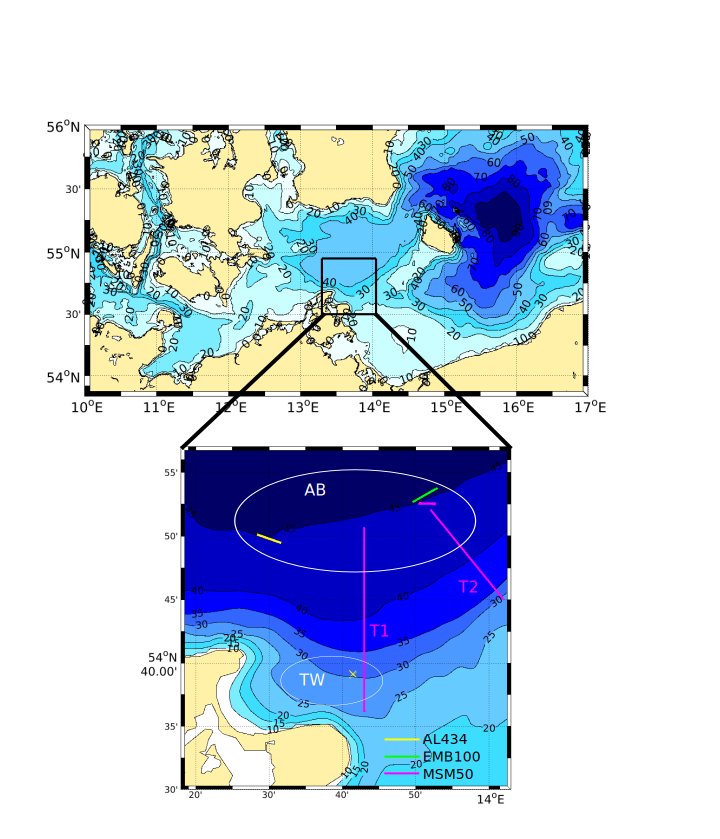
\includegraphics[width=18cm]{bilder/studyarea.pdf}
 \caption{Bathymetric map of the Western Baltic Sea and an enlargement of the 
study area. Deployments during cruise AL434 are indicated in yellow, from 
EMB100 in green and from cruise MSM50 in magenta.}
 \label{studyarea}
 \end{figure}

Two main drivers are determining the currents. From the exchange with the North 
Sea, dense bottom currents of saline water flows into the Arkona Basin. 
Coriolis effects form a topographically trapped dense rim current which rotates 
cyclonically around the basin, following the slope. As inflow events are 
driven by larger scale wind forcing, this process is not steady, and the 
dense bottom current can disappear completely. Parts of the saline bottom water 
are transferred from the cyclonic bottom current to the saline bottom water 
pool, which fills approximately the lowermost 15~m of the basin. The barotropic 
cyclonic motion performs basin wide zonal oscillations on timescales of one 
week \citep[][]{lass2003}.

Near-shore currents reveal an elliptical motions, with the main axis 
being aligned along the isobaths \citep[][]{lass2003}. North of the island 
R\"{u}gen, the currents are slightly more pronounced towards the east. The 
cross-shore component is generally weaker, but still in the order of 
0.1~m~s$^{-1}$ \citep[][]{lass1993}. 

The other main factor determining the flow conditions is local wind forcing, 
that causes upwelling and downwelling near the shore. Wind from the east drives 
a long-shore current to the west. In cross-shore direction, Ekman 
transport causes surface flow to be directed seaward. This induces a 
near-bottom return current towards the land \citep[][]{lass1993}. The salt 
water pool in the Arkona basin is consequently tilted upwards towards the 
southern rim of the basin \citep[][]{lass2003}. During wind from the west, the 
situation is reversed. 

 \FloatBarrier
\subsection{Sedimentology}

  Sediment distribution in this area is heterogeneous in the shallow regions 
with predominately medium to fine sand. At water depths below 25 - 30~m in the 
Arkona Basin, sediment is finer and consists homogeneously of silt 
(\fig{tauberkarte}). In the vicinity of TW, a special type of fine grained and 
organic poor sediment is found. Previous studies \citep[][]{leipe2000, 
basys1} found the Arkona Basin to be a deposition center for material 
orginiating from the shallower areas, with accumulation rates of around 2.2 
mm/yr. Sediment characteristics in the Arkona Basin resemble to those of a 
fluffy layer, i.e. it is easily resuspended and, due to its low settling 
velocity, remains suspended for a relatively long period of time. A consecutive 
study \citep[][]{basys2} found the 20~m isobath to be the border between 
erosional and depositional sites in this area, yielding that the Tromper Wiek 
region is depositional as well. This study also pointed out that muddy 
sediments accumulated below the halocline in this region.
 \begin{figure}[ht]
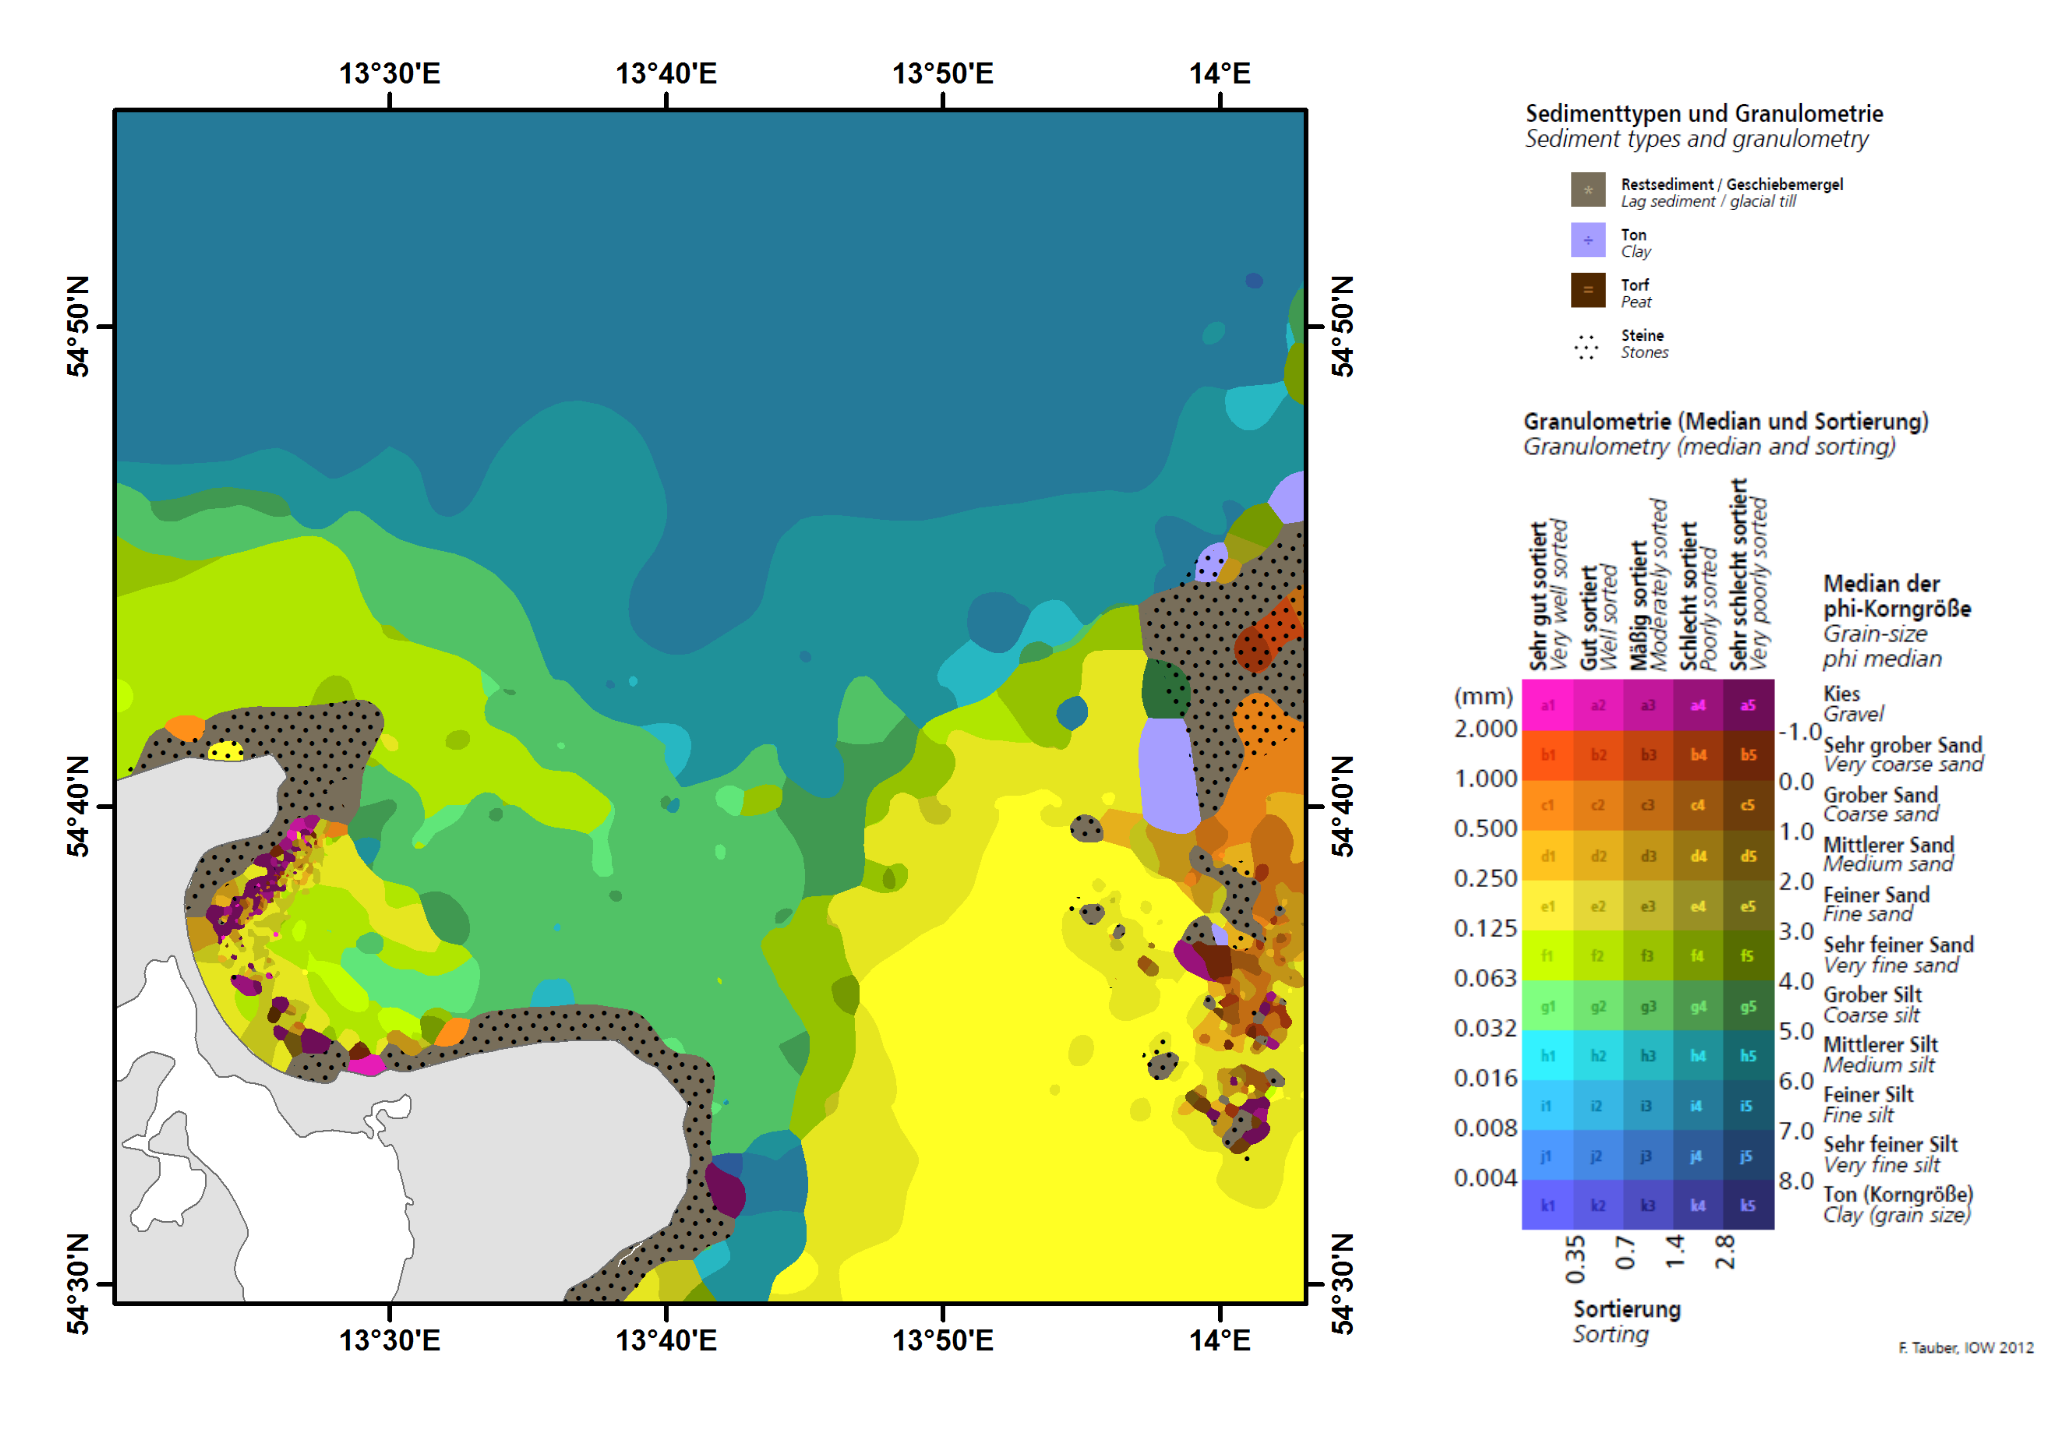
\includegraphics[width=30pc]{bilder/TW.pdf}
 \caption{Sediment distribution in the study area. Data were taken from 
\cite{tauber2012}.}
 \label{tauberkarte}
 \end{figure}

\section{Instrumentation}

We obtained hydrographic and turbulence data at 
several locations throughout the German coastal area during three cruises with 
R/V \textit{Alkor} in spring 2014 (AL434, 28.03.-08.04.2014), R/V 
\textit{Elisabeth Mann Borgese} in spring 2015 (EMB100, 09.04.-16.04.2015) and 
R/V \textit{Maria S. Merian} in winter 2016 (MSM50, 05.01.-29.01.2016). Here, 
we exclusively discuss data obtained in the transition zone from the coast off 
the island R\"{u}gen (called Tromper Wiek (TW), around 30~m water depth) to 
the approximately 45~m deep Arkona Basin (AB). The exact positions of deployed 
moorings and ship-based microstructure profiler transects are indicated in 
\fig{studyarea}.

Three different types of moorings were deployed: A CTD-Chain consisted of eight 
CTD-loggers (MicroCat from Seabird, USA), tied to a mooring line at intervals 
of 1 m, starting at 1 m above the seabed, additionally two optical 
backscatter sensors (NTU from Wetlabs, USA) at 3.5 and 5.5 m above the seabed. 
For the EMB100 cruise, the CTD-Chain was extended to 10 CTD-loggers (5 MicroCat 
and 5 TR-1060 type from RBR, Canada) and the turbidity sensors were omitted. 
Lander 1 was a bottom-mounted instrument frame with an upward looking 1200 kHz 
ADCP (Teledyne RDI, USA), a 6 MHz single-point Doppler current meter (Vector 
from Nortek AS, Norway), another CTD-logger and a turbidity sensor. Lander 2 
was a similar bottom frame equipped with an upward looking 600 MHz ADCP 
(Teledyne RDI, USA) and an upward looking 1 MHz (2 MHz during cruise AL434) 
pulse-coherent ADCP (Aquadopp HR from Nortek AS, Norway). For the cruises 
EMB100 and MSM50, Lander 2 was complemented with an additional CTD-logger and a 
turbidity sensor. Deployment times of the moorings are listed in 
\tab{deployments}.

 \begin{table}
\caption{Deployment times of moorings (UTC). In the first 
line, TW and AB indicate deployment sites near the coast and in the Arkona 
Basin, respectively.}\label{deployments}
\begin{center}
\begin{tabular}{cccc}
 & AL434 (TW) & EMB100 (AB) & MSM50 (TW) \\
 \hline
 start & 03.04.2014, 07:00 & 14.04.2015, 12:00 & 26.01.2016, 22:00 \\ 
 end & 08.04.2014, 06:00 & 17.04.2015 04:00 & 28.01.2016, 07:00 \\
\hline
 & CTD-Chain & CTD-Chain & \\
 & Lander 1 & Lander 1 & Lander 1\\
 & Lander 2 & Lander 2 & Lander 2\\
\end{tabular}
\end{center}
\end{table}

Ship-based microstructure measurements were performed with a MSS90-L 
microstructure profiler (ISW, Germany). The instrument contained a set of 
precision CTD sensors, a fast FP07 thermistor, a turbidity sensor, and two 
airfoil shear-probes. During the transects (each of 1 to 5 hours duration) the 
ship moved at 1-2 kn and profiles were obtained continously. Number and time of 
the transects for each cruise are summarized in \tab{mss}.

 \begin{table}
\caption{Start and end times (UTC) and number (in brackets) of microstructure 
transects.}\label{mss}
\begin{center}
\begin{tabular}{cccc}
 & AL434 (2014) & EMB100 (2015) & MSM50 (2016)\\
 \hline
Tromper & 04.04., 16:15 - & & 27.01., 00:00 - \\ 
Wiek & 04.04., 22:30 (4) & & 28.01., 06:00 (9)\\
 & 06.04., 17:30 & & \\
 &  07.04., 22:15 (8) & & \\
\hline
Arkona & 05.04., 16:15 - & 14.04., 16:45 - & 23.01., 13:30 - \\
Basin & 06.04., 01:15 (5) & 15.04., 05:30 (5) & 24.01., 16:45 (7)\\
\hline
transect &  & & 24.01., 19:30 - 23:45 (T1)\\
coast to basin & & & 28.01., 09:45 - 17:00 (T2)\\
\end{tabular}
\end{center}
\end{table}

\section{Observations}

\subsection{Tromper Wiek}

During the 5 day instrument deployment in 2014 (\tab{deployments}), we captured 
a storm event with 7 Bft wind and up to 4 m wave height with a consecutive calm 
period (\fig{tromperwiek}, a). In \fig{tromperwiek}, b the variance of the 
horizontal velocity componentsfiltered for wave periods between 2 and 20 
seconds, which is proportional to the kinetic energy contained in the 
waves, is displayed. Although wave energy was maximal in the afternoon of April 
4, the peak in turbidity was not reached until late morning of April, 5. This 
yields that local resuspension during storm did not occur, but a turbid 
watermass was advected to the measurement site. Near bottom current 
(\fig{tromperwiek},c) was directed to the south during the relevant period, 
i.e. water from deeper parts was advected up the slope.

 \begin{figure}[ht]
\includegraphics[width=15cm]{bilder/al434tw.pdf}
 \caption{(A) Wind speed and direction from the hindcast of the German Weather 
Service, (B) wave energy and turbidity and (C) direction of 
near bottom current, all obtained with Lander 1 during the deployment at TW on 
cruise AL434 (April 2014).}
 \label{tromperwiek}
 \end{figure}
 
 This advection of saline water near the bottom is triggered by the local wind 
forcing. Strong easterly wind causes Ekman transport to the north (i.e. 
offshore) in the surface layer \citep[][]{lass2001}, which is visible in the 
velocity data from the 600~kHz ADCP mounted on Lander~2, displayed in 
\fig{adcp600}. The distorted values in the uppermost part of the water column 
during April 4 coincide with the periods of time during which surface waves 
could be recorded with the ADV. They originate from breaking waves which 
disrupt the acoustic velocity measurements. The near-bottom return current below 
17~m depth is rather oscillatory than steady, but exhibits a trend to southerly 
(i.e. onshore) directions during the storm. Maximal onshore bottom flow is 
reached by the beginning of April 5. After the wind decayed and changed 
direction to westerly wind at the end of April 5, the surface current 
firstly decayed and was then reversed to flow approximately southwards. The 
near-bottom current of the flow remained unsteady, but was generally directed 
eastwards. This is more clearly visible from \fig{tromperwiek},c.

 \begin{figure}[ht]
\includegraphics[width=40pc]{bilder/adcp600.png}
 \caption{Time series of velocity profiles obtained with the 600~kHz ADCP on 
Lander 2 during the deployment at TW on cruise AL434 (April 2014).}
 \label{adcp600}
 \end{figure}

 In the CTD Chain data in \fig{ctdchain}, where salinity in the lowermost 8~m 
of the water column is displayed, we see an increase of the 
near-bottom salinity, accompanied by increasing turbidity, starting in the 
afternoon of April 4. The increase in turbidity is clearly linked to the 
increase of salinity, supporting that turbid water is advected to TW from deeper 
regions. Furthermore, salinity data in the record reaches a level that 
resembles more to the saline bottom water in the Arkona basin below the 
halocline than to the brackish surface water. This indicates that upwelling 
tilted the halocline towards the south and saline bottom water reached far 
upslope to the shore.

 \begin{figure}[ht]
\includegraphics[width=15cm]{bilder/ctdchaintw.png}
 \caption{Salinity data obtained from the CTD Chain deployed at TW 
during cruise AL434 (see \tab{deployments}).}
 \label{ctdchain}
 \end{figure}

 
\FloatBarrier
\subsection{Basin to Coast Transect}

In \fig{transect} we see how the water body is structured along the slope from 
the coast into the basin. A sharp halocline seperates a turbulent bottom 
boundary layer (BBL) of approximately 5~m thickness from the interior. At the 
left hand side, where the slope angle steepens, the halocline is widened where 
it approaches the sea floor. 

The boundary layer is generally turbid. Turbidity is more patchy towards the 
shallow areas, but high values are confined to the bottom boundary layer, 
so no suspended matter is mixed across the halocline. This indicates that 
turbidity is caused by material originating from the sea floor and held in 
suspension by turbulent motions in the BBL.

Just like turbidity, dissipation is also enhanced in the BBL. In the area where 
the halocline encounters the sea bed on the steep slope, dissipation is 
suppressed by the high stratification. Further up the slope, right above the 
halocline, there is again an area with greatly enhanced dissipation. This 
yields that sediment could be resuspended locally when the halocline is 
advected up the slope.

Isolines of salinity (please note that salinity determines the density in this 
region) below the halocline are tilted towards the bottom, consistent with the 
observations of boundary layers over sloping topography in e.g. 
\cite{Lorkeetal2005a}. Shear induced convection and, in the presence of an 
oscillatory current, residual (upslope) sediment transport as described in 
\cite{schulzumlauf2016} is consequently within the realms of possibility here.

\begin{figure}[ht]
\includegraphics[width=40pc]{bilder/abtrans.png}
 \caption{Turbidity and dissipation rate from the microstructure transect T1 
in January 2016. White lines indicate levels of equal salinity.}
 \label{transect}
 \end{figure}

\FloatBarrier
\subsection{Arkona Basin}

 During each of the three cruises, we collected microstructure data in the 
Arkona Basin. \fig{abmss} shows the profiles of dissipation rate and turbidity, 
averaged over all profiles obtained in the basin for each cruise. A turbulent 
BBL is visible in all three profiles, ranging from 1 to 5 m thickness. 
Turbidity is again enhanced in the BBL, but not above, supporting the 
observation from the last section. As this data set was obtained over three 
years and in different seasons, it is most likely that this turbid, very 
sharply defined BBL is constantly present in the Arkona Basin.

   \begin{figure}[ht]
\includegraphics[width=15cm]{bilder/arkona_mss.pdf}
 \caption{Turbidity and dissipation rate from all microstructure transect in 
the Arkona Basin. Solid lines are mean values, dashed line the standard 
deviation. Only the lowermost part of the watercolumn is displayed here.}
 \label{abmss}
 \end{figure}

The data described in the sections above yields that this reservoir of fine 
grained sediment, constantly held in suspension, can be advectively 
transported across the rim of the Arkona basin to the shallower areas well 
below 30~m. 

\section{Discussion and Conclusions}

This study focusses on finding processes which can transport sediment upslope 
from the deep basins back to shallower areas. We have found from the 
microstructure measurements in the Arkona basin, that in spite of the depth and 
therefore the absence of wave-induced resuspension, a layer of 
suspended fine-grained sediment is present near the bottom. We furthermore 
found, that this turbid and turbulent BBL is present everywhere along the 
slope, confined by a regional halocline. 
\chapter{The Effect of Wind Waves on Sediment Properties}
\label{kap-waves}

Wind generated waves are a main contributor to the energetics in shallow water 
bodies. They generate surface mixed layers and influence the near bed dynamics 
even at considerable water depths. In shallow areas, wave induced maximal 
bottom stress mainly dominates over current induced turbulence 
\citep[][]{jonsson2004}. Consequently, waves play a major role in sediment 
transport and distribution in the Baltic Sea.

\section{Introduction}

DEFINITION PERMEABILITY. Sediments that are considered as permeable allow pore 
water flow and exchange by hydrodynamically imposed pressure differences. 
Biogeochemical processes in the sediment are strongly affected by this process, 
and potentially permeable sediments are present in estimately 70$\%$ of the 
global shelf seas. CITE EMERY1968

Permeability is related to grain size distribution and size and geometry of the 
interstices in the sediment. 



\section{Permeability Map}

\cite{forster2003} constructed a map reflecting the permeability in the western 
Baltic Sea using direct measurements of vertical permeability and estimates 
from grain size distribution and porosity. From 37 samples, hydraulic 
conductivity was measured and converted to permeability. From the same samples, 
grain size distribution was determined. An approximation for the permeability 
is the relation of Krumbein and Monk \citep[][]{krumbein1942}
\begin{equation}
 \label{kKM}
 k_{KM} = 7.5 \times 10^{-4} d_{50}^2 e^{-1.31 \sigma},
\end{equation}
where $d_{50}$ is the median diameter and $\sigma$ the standard deviation of 
the grain size distribution. This relation only holds for sufficiently well 
sorted sediments with $\sigma \leq 0.7$. This formula was found to overestimate 
the permeability, thus Eq.\ref{kKM} was divided by a correction factor of 2.6.  
With this new relation, permeability was estimated from two data sets of grain 
size distribution and interpolated. The data are shown in Fig.\ref{perm}.
\begin{figure}[ht]
 \includegraphics[width=16cm]{bilder/perm_k.png}
 \caption{Permeability data from \cite{forster2003}. Reprinted 
with permission. Pink line indicates the k=$2.5\times10^{-12}$ 
isoline.\label{perm}}
\end{figure}

\section{Wave model for the Baltic Sea}\label{balticswan}

The SWAN wave model version 41.01 was set up for the Baltic Sea including a 
nesting in the area of the German coastal sea. For the whole Baltic Sea, a grid 
resolution of $0.5^\circ \times 0.1^\circ $ in Latitude and Longitude was chosen 
in a domain reaching from $53.5^\circ \text{N } 9^\circ \text{E}$ to $66^\circ 
\text{N } 31^\circ \text{E}$. This includes the Kattegat, the passage from the 
Baltic to the North Sea, where boundary conditions were prescribed in the east: 
A constant JONSWAP spectrum with a wave height of $1$ m, a period of $5$ s and 
peak wave direction of $90^\circ$ with a high directional spreading. The passage 
from the North to the Baltic sea is very shallow, so the boundary conditions 
have negligible influence on the model outcome. Wave frequency range was set to 
0.1 to 1.8 Hz, which mirrors the actual wave frequencies in the Baltic 
Sea \citep[][]{balticsea}, with a resolution of $42$ frequency bins. 
Computations included a spin-up time of $10$ days, sufficient for wave modeling 
and were performed for the years 2013 and 2014. The model was forced by wind 
data from the German Weather Service (DWD), the computational time step was $1$ 
hour (note that the propagation scheme implemented in SWAN is implicit, so the 
time step is not restricted by numerical issues). 

The nesting area reached from $53.5^\circ \text{N } 10^\circ \text{E}$ to 
$55.5^\circ \text{N } 15^\circ \text{E}$, including the Western German coastal 
seas. Spatial resolution was $0.01^\circ \times 0.025^\circ $ in Latitude and 
Longitude and the computational time step was set to $15$ minutes. Boundary 
conditions came from the Baltic Sea model and all parameters were left 
unchanged.

In \fig{verify} the significant wave height calculated with the wave model was 
compared to data obtained with a wave rider buoy. The significant wave height 
is defined as the average wave height of the highest one-third of the waves. 
This value matches the visually observed wave height best and can be calculated 
from the zeroth-order moment if the variance density spectrum $m_0$ via 
$H_{sign} = 4 \sqrt{m_0}$.
\begin{figure}[ht]
 \includegraphics[width=9cm]{bilder/januar.pdf}
 \caption{Significant wave height calculated with the SWAN wave model (HR 
refers to the high resolved nested run) and measured wave height from the 
Arkona wave rider buoy.\label{verify}}
\end{figure}

In the context of a Master Thesis \citep[][]{masterarbeitronja}, the model 
setup for 2013 (still using the previous version SWAN 40.91AB) was 
extensively tested for numerical convergence and compared to measured data on 
several locations in the Baltic Sea. Wave parameters like significant wave 
height were in good agreement with obtained data, even in areas with complex 
topography. A brief description of wind wave properties and processes and a 
discussion the wave model SWAN can be found in Appendix B.

\subsection{Idealized Wind Situations}

Storm surges in the Baltic sea are caused by two large-scale wheater 
situations. Strong northwest or northeast winds generate the highest 
waves in the western Baltic \citep[][]{balticsea}. Northeast winds maximize the 
fetch and therefore the wave activity in German coastal waters. Strong 
northwesterly winds occur more frequently, but tend to last shorter. 

To model wave activity under the two scenarios described above, we forced the 
Baltic Sea wave model with constant wind from the northwest (NW) and the 
northeast (NE), respectively. Wind speed was set to 20 m~s$^{-1}$, which was 
the maximal wind speed reached during a strong northwest wind in January 2005.
We used the same resolution and configuration as described in 
section \ref{balticswan} and a the modeled time period sufficiently long to 
reach stationarity (10 days).

\section{Results}	

\section{Discussion}

\section{Conclusions}
\end{mainmatter}

% Anhaenge -- auskommentieren falls nicht ben\"{o}tigt.
\begin{appendices}
\chapter{Numerical boundary conditions for SPM concentrations}
\pagenumbering{roman}

In view of the strong near-bottom gradients of suspended material, the
implementation of the boundary conditions for the SPM transport
equation \eq{c} requires special attention. While \eq{defFz} provides
an exact expression for the upward turbulent flux $F_z$ at the bottom,
the numerical implementation of the sinking flux,
\begin{equation}
 \label{Fs}
 F_s(z=0) = w_s c_0 \comma
\end{equation}
is not straightforward because the bottom concentration, $c_0$, is
unknown. In vertically staggered numerical grids typically used in
ocean modeling, the bottom concentration $c_0$ has to be estimated
from the known concentration $c_1$ in the center of the lowermost grid
cell, which requires some assumptions about the vertical distribution
of the suspended material in the near-bottom region. While it is
reasonable to assume that the bottom cell is well mixed (i.e.,
$c_0=c_1$) if the bed stress $|\tau_b|$ is smaller than the critical
stress for erosion, $\tau_c$, it is likely that the bottom
concentration $c_0$ is significantly larger than $c_1$ if active
erosion takes place ($|\tau_b| > \tau_c$). In this case, the popular
assumption $c_0=c_1$ may lead to large numerical errors, and to a grid
dependence of the numerical solution. In the following, we show how a
more consistent lower boundary condition can be derived.

We start from the observation that close to the bottom, the transport
equation in \eq{c} reduces to a balance between upward mixing and
downward sinking of suspended material,
\begin{equation}
 \label{cstationary}
 0 = \nu_t^b \partder{c}{z} + w_s c
 \comma
\end{equation}
assuming small slopes ($\alpha \ll 1$) for simplicity. The turbulent
viscosity in the near-bottom region is known to follow the
law-of-the-wall relation $\nu_t = \kappa u_\ast (z + z_0)$, where
$\kappa \approx 0.4$ is the von K{\'a}rm{\'a}n constant, and $u_\ast =
|\tau_b|^{1/2}$ the bottom friction velocity
\citep[e.g.,][]{Pope2000a}. The turbulent diffusivity $\nu_t^b$ in this
region is proportional to $\nu_t$, and therefore adopts the form
$\nu_t^b = Pr_t^{-1} \kappa u_\ast (z + z_0)$, where the turbulent
Prandtl number, $Pr_t$, plays the role of a constant proportionality
factor of order 1. The turbulence model used in our study has been shown to
exactly reproduce this near-wall behavior for $\nu_t$ and $\nu_t^b$
\citep[e.g., ][]{UmlaufBurchard2003a,UmlaufBurchard2005a}.

Inserting the above law-of-the-wall relation for $\nu_t^b$ into
\eq{cstationary}, we find a solution of the form
\begin{equation}
 \label{Rouse}
 \dfrac{c}{c_0} = \left( \frac{z}{z_0} + 1 \right)^{-p} \comma
\end{equation}
which is recognized as the classical Rouse profile
\citep{vanRijn84b}, slightly modified here by the appearance of the
turbulent Prandtl number in the definition of the Rouse number $p =
w_sPr_t \, / (\kappa u_\ast)$.

Recalling that in any conservative numerical scheme, $c_1$ represents
the average concentration inside the lowermost grid cell, a relation
between $c_0$ and $c_1$ may be found from integrating \eq{Rouse}
across the cell. If we denote $h$ as the cell thickness, this yields
\begin{equation}
 \label{cbot}
 c_0 = \frac{c_1}{r} \quad \text{for} \quad |\tau_b|>\tau_c \comma
\end{equation}
where 
\begin{equation}
 \label{rr}
 r =  \frac{1}{(1-p) h/z_0} \left[ \left( \frac{h}{z_0} + 1 \right)^{1-p} -1 \right] 
 \comma
\end{equation}
\begin{figure}[h]
  \noindent\includegraphics[width=29pc,angle=0]{bilder/rouse.pdf}\\
  \caption{A1}{Concentration ratio $c_1/c_0$ as a function of
    non-dimensional cell thickness, $h/z_0$, for different Rouse
    numbers according to \eq{cbot}.\label{c0c1}}
\end{figure}
Fig. A1 shows the ratio $r=c_1/c_0$ as a function of the normalized
cell thickness $h/z_0$ for different Rouse numbers. The most important
conclusion from this figure is that the naive approach of assuming
$c_0 = c_1$ to compute the sinking flux in \eq{Fs} during erosion
periods introduces large numerical errors except for small Rouse
numbers and/or extremely fine grids with $h \ll z_0$. Below, we
nevertheless discuss some reference solutions that satisfy this
condition. We note, however, that the constraint $h \ll z_0$ implies
$\Delta t \ll z_0 / w_s$ for the numerical time step according to the
well-known CFL stability criterion for explicit advection schemes. It
is easy to show that, even for idealized one-dimensional simulations,
the numerical effort may become prohibitively large for small $z_0$.

Using the example from Section \ref{sec:bbl} above, Fig. A2
illustrates that assuming $c_0 = c_1$ during both erosive and
non-erosive periods leads to significant numerical errors, and to a
grid-dependence of the results. 
\begin{figure}[h]
  \noindent\includegraphics[width=29pc,angle=0]{bilder/appendix.pdf}\\ \caption{A2}{Numerical
    results for (a) SPM concentration 5~m above the bottom, and (b)
    upslope flux $F_x$ for three vertical resolutions. Gray lines are
    based on the assumption $c_0 = c_1$ to compute the sinking flux in
    \eq{Fs}, whereas black lines are based on \eq{cbot} during erosive
    periods. Parameters correspond to Case 1 in
    \tab{params}. \label{convergence}}
\end{figure}
Estimating $c_0$ based on \eq{cbot}
during periods with active erosion, however, removes this dependency
on the numerical grid, and leads to stable results already for
moderate vertical resolution. All results discussed in this manuscript
are therefore based on this new expression. Convergence studies were
carried out to insure that all our results are independent of the
numerical grid size and time step.
\end{appendices}

\begin{backmatter}
% Verweis auf Literaturverzeichnis zum Inhaltsverzeichnis hinzufuegen
\addtocontents{toc}{\vspace*{1em}}

% Literaturliste aus Literaturdatenbank (Bibtex-Datei) bauen. Nur tatsaechlich zitierte Literatur wird in Liste aufgenommen.
% Regelmaessigen Aufruf von ``bibtex abschlussarbeit'' nicht vergessen, falls das der Latex-Editor nicht
% erledigt.
% Zur Bearbeitung der Literaturdatenbank kann das Programm JabRef (http://jabref.sf.net) empfohlen werden. (Java-Programm, laeuft unter Windows, Linux, Mac, ...)
\bibliography{literatur}
% Stil fuer Literaturliste festlegen
% Variante A: DIN, Eintraege erhalten Kuerzel aus Autoren-Initialien und Jahr, alphabetisch geordnet
% \bibliographystyle{alphadin}
% Variante B: DIN, Eintraege werden durchnummeriert, alphabetisch geordnet
\bibliographystyle{ametsoc2014}


\begin{abstract}[Selbständigkeitserklärung]
\thispagestyle{empty}
Ich versichere hiermit an Eides statt, dass ich die vorliegende Arbeit selbstständig
angefertigt und ohne fremde Hilfe verfasst habe, keine außer den von mir
angegebenen Hilfsmitteln und Quellen dazu verwendet habe und die den benutzten
Werken inhaltlich und wörtlich entnommenen Stellen als solche kenntlich gemacht
habe.
\vspace*{2cm}

\flushright{
Rostock, 07. Oktober 2016
}
\end{abstract}

\end{backmatter}

\end{document}
